\chapter{関連研究}
\section{行動情報から心的状態を推定する研究}
\par
行動情報から心的状態を推定する研究として,人間の心的状態理論Theory of Mind(ToM)をベイズ推論を用いてモデル化するBToM\cite{baker2011bayesian}が存在する.BToMは,環境の状態や人間の心的状態を部分的に観測可能なマルコフ決定過程(POMDP)として表し,環境における人間の行動をベイズ推論に適用することで,人間が観測できていない環境領域についての信念と欲求を共同推定する.人間の信念と欲求を共同推定することで,信念と欲求の相互作用を捉えることができる.図\ref{fig:btom}に,BToMにおけるベイズ推論の様子を示す.
\begin{figure}[htbp]
  \begin{center}
    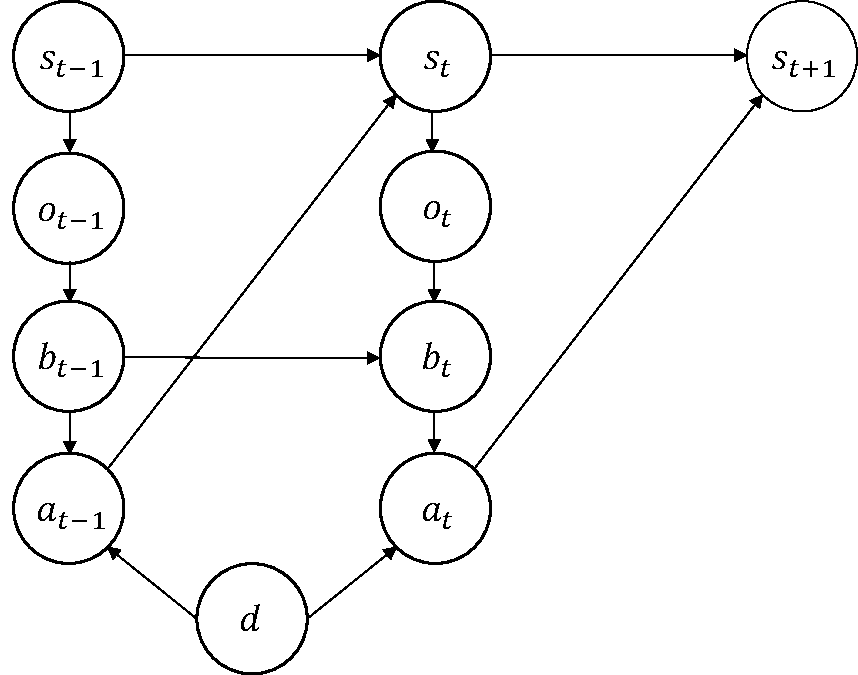
\includegraphics[scale=0.85]{./btom.pdf}
    \caption{BToMにおけるベイズ推論の様子}
    \label{fig:btom}
  \end{center}
\end{figure}
BToMにおけるベイズ推定では,時刻$t$における環境の状態$s_{t}$を基に人間の観測状況$o_{t}$が計算される.また,$o_{t}$を基に人間の信念$b_{t}$が計算され,$b_{t}$と人間の欲求$d$から人間の行動$a_{t}$が計算される.$a_{t}$が起こることにより,環境の状態は$s_{t+1}$に変化し,人間の観測状況,信念および行動が再起的に計算される.BToMでは,$P(b_t,d|s_{1:t},a_{1:t-1})$を解くことを目的としている.ここで,$s_{1:t}$は,時刻$1$から時刻$t$までの環境の状態遷移,$a_{1:t-1}$は,時刻$1$から時刻$t-1$までの人間の行動履歴,$P(b_t,d|s_{1:t},a_{1:t-1})$は,$s_{1:t}$および$a_{1:t-1}$から計算される$b_t$と$d$の確率である.以下に,$P(b_t,d|s_{1:t},a_{1:t-1})$にベイズの定理を適用した過程を示す.
\begin{equation}
  \begin{split}
  \label{btom}
  P(b_t,d|s_{1:t},a_{1:t-1}) &\propto P(b_t,d,s_{1:t},a_{1:t-1})\\
  &= \sum_{b_{t-1},o_t}P(b_t,d,s_{1:t},a_{1:t-1},b_{t-1},o_t)\\
  &= \sum_{b_{t-1},o_t}P(b_t|d,s_{1:t},a_{1:t-1},b_{t-1},o_t)\cdot P(d,s_{1:t},a_{1:t-1},b_{t-1},o_t)\\
  &= \sum_{b_{t-1},o_t}P(b_t|b_{t-1},o_t)\cdot P(o_t|d,s_{1:t},a_{1:t-1},b_{t-1})\cdot P(d,s_{1:t},a_{1:t-1},b_{t-1})\\
  &= \sum_{b_{t-1},o_t}P(b_t|b_{t-1},o_t)\cdot P(o_t|s_t)\cdot P(s_t|s_{t-1},a_{t-1})\\
  &\hspace{3cm} \cdot P(a_{t-1}|b_{t-1},d)\cdot P(b_{t-1},d,s_{t-1},a_{t-2})\\
  \end{split}
\end{equation}
ここで,$P(b_t|b_{t-1},o_t)$は人間の観測$o_t$によって信念$b_t$が更新される確率,$P(o_t|s_t)$は環境の状態$s_t$において人間が観測状況$o_t$を得る確率,$P(s_t|s_{t-1},a_{t-1})$は環境の状態$s_{t-1}$において,人間が行動$a_{t-1}$を起こした時に環境の状態が$s_t$になる確率,$P(a_{t-1}|b_{t-1},d)$は人間が信念$b_{t-1}$,欲求$d$を持っている時に行動$a_{t-1}$を起こす確率,$P(b_{t-1},d,s_{t-1},a_{t-2})$は時刻$t-1$におけるBToMの出力である.
式(\ref{btom})より,$P(b_t,d|s_{1:t},a_{1:t-1})$は再起関数として表すことができ,初期値$P(b_1,d,s_1,a_0)$を決めることで更新することができる.


\par
運転状況から心的状態を推定する研究\cite{darwish2020learning}も存在する.運転は,運転者によりスピードや前方車との車間距離が異なる.また,天候や時間によって運転手がとる行動は変化する.運転者がどのような行動をとることを意図しているかを推定するために,交通状況を部分的に観測可能なマルコフ決定過程として表し,運転者の心的状態をBToMを用いてモデル化している.その結果,自動運転において運転者の意図に沿った動作の実現を手助けする.

\par
また,作業用ロボットに行動情報と心的状態の関係を適用した研究\cite{inbook}も存在する.人間の作業員のアシスタントとして,人間の意図推定できるロボットを導入することで,効率的かつ安全な作業を行うことを目的としている.人間の行動から意図を推定する.人間の心的状態の移り変わりも考慮している.

\section{言語情報から心的状態を推定する研究}
\par
言語情報から心的状態を推定する研究として,発話から信念や欲求,意図を推定する研究\cite{高橋拓誠2015bdi}がある.意図を持った対話を行う対話システムの実現のために,信念と欲求を推定し,意図が生成される.BDIモデルは,Beliefモジュール,Desireモジュール,Intentionモジュールから構成される.最初に,Beliefモジュールにおいて発話から事象を抽出し,信念として捉える.Desireモジュールでは,Beliefモジュールにおいて捉えられた信念を基に欲求の候補を複数生成する.また,生成された欲求の候補に対し,情緒生起手法\cite{2002}を適用し,それぞれの尤度を算出し,最も尤度が高いものを欲求とする.Intentionモジュールでは,Desireモジュールにおいて選択された欲求を基に意図生成を行う.

\par
また,検索精度向上のために,入力クエリに含まれる言語情報からユーザの心的状態を推定する研究\cite{10.1007/978-3-642-02481-8_4}も存在する.

\section{単一情報心的状態推定の問題点}
\par
人間同士の対話では,行動によって発話の解釈が変わったり,発話によって行動の解釈が変わることは少なくない.対話システムと人間との対話においても,行動によって発話の解釈を変えたり,発話によって行動の解釈を変えるために行動情報と発話情報の両方を活用した心的状態の推定が重要である.しかし上記の研究は,いずれも行動情報もしくは発話情報を含む言語情報の一方のみを心的状態の推定に活用したものである.これらの推定は,行動情報のみを観測できる場合や発話情報のみを観測できる場合には有効であるが,行動情報と発話情報の両方を観測できる場合においては不十分である.行動情報と発話情報の一方のみの単一情報による心的状態の推定では,行動による発話の解釈の変化や発話による行動の解釈の変化を捉えることができず,行動情報と発話情報の相互作用を考慮して心的状態を推定することができない.
